\documentclass[12pt]{article}
\usepackage{tikz}
\usepackage{amsmath}
\usepackage{geometry}
\geometry{a4paper, margin=1in}
\usetikzlibrary{arrows.meta, positioning, decorations.pathreplacing}

\tikzset{
	box/.style={draw, thick, minimum size=6mm, inner sep=0pt},
	base/.style={box, fill=blue!20},
	slope/.style={box, fill=red!20},
	normal/.style={box, fill=gray!10}
}

\begin{document}
	
	\section*{4. The Grand Cancellation: Why the $q^6$ term is 0}
	
	Let's look at all partitions of $6$ into distinct parts. There are exactly 4 valid partitions: $6$, $5+1$, $4+2$, and $3+2+1$. 
	Franklin's involution pairs them up perfectly. The block that moves is highlighted: \textbf{Red} when it moves from the Slope, and \textbf{Blue} when it moves from the Base.
	
	\vspace{1cm}
	\begin{center}
		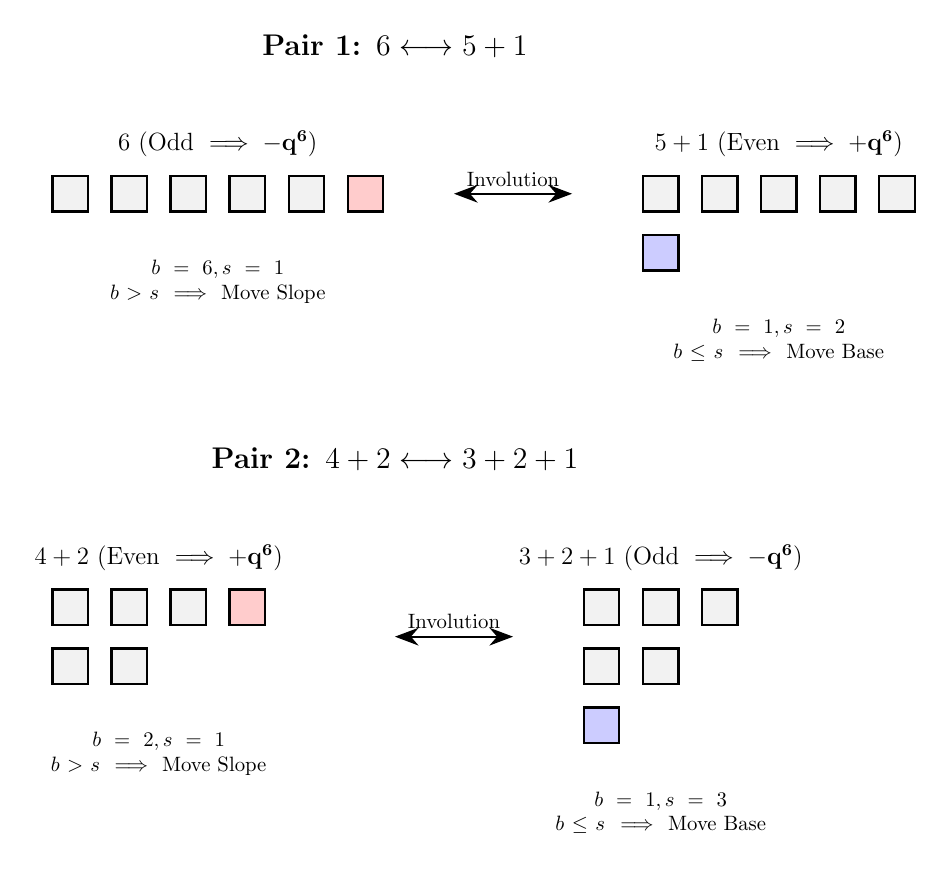
\begin{tikzpicture}[scale=0.75, transform shape]
			
			% ==========================================
			% PAIR 1: 6 <--> 5 + 1
			% ==========================================
			\node[font=\Large\bfseries] at (5.5, 2.5) {Pair 1: $6 \longleftrightarrow 5+1$};
			
			% --- Partition 6 ---
			\begin{scope}[shift={(0,0)}]
				\node[above, font=\large] at (2.5, 0.5) {$6$ (Odd $\implies \mathbf{-q^6}$)};
				\foreach \x in {0,1,2,3,4} \node[normal] at (\x, 0) {};
				\node[slope] at (5, 0) {}; % The slope block
				\node[below, text width=4cm, align=center] at (2.5, -1) {$b=6, s=1$\\$b > s \implies$ Move Slope};
			\end{scope}
			
			% Involution Arrow
			\draw[{Stealth[length=3mm]}-{Stealth[length=3mm]}, thick] (6.5, 0) -- node[above] {Involution} (8.5, 0);
			
			% --- Partition 5 + 1 ---
			\begin{scope}[shift={(10,0)}]
				\node[above, font=\large] at (2, 0.5) {$5+1$ (Even $\implies \mathbf{+q^6}$)};
				\foreach \x in {0,1,2,3,4} \node[normal] at (\x, 0) {};
				\node[base] at (0, -1) {}; % The base block
				\node[below, text width=4cm, align=center] at (2, -2) {$b=1, s=2$\\$b \le s \implies$ Move Base};
			\end{scope}
			
			
			% ==========================================
			% PAIR 2: 4 + 2 <--> 3 + 2 + 1
			% ==========================================
			\node[font=\Large\bfseries] at (5.5, -4.5) {Pair 2: $4+2 \longleftrightarrow 3+2+1$};
			
			% --- Partition 4 + 2 ---
			\begin{scope}[shift={(0,-7)}]
				\node[above, font=\large] at (1.5, 0.5) {$4+2$ (Even $\implies \mathbf{+q^6}$)};
				\foreach \x in {0,1,2} \node[normal] at (\x, 0) {};
				\node[slope] at (3, 0) {}; % The slope block
				\foreach \x in {0,1} \node[normal] at (\x, -1) {};
				\node[below, text width=4cm, align=center] at (1.5, -2) {$b=2, s=1$\\$b > s \implies$ Move Slope};
			\end{scope}
			
			% Involution Arrow
			\draw[{Stealth[length=3mm]}-{Stealth[length=3mm]}, thick] (5.5, -7.5) -- node[above] {Involution} (7.5, -7.5);
			
			% --- Partition 3 + 2 + 1 ---
			\begin{scope}[shift={(9,-7)}]
				\node[above, font=\large] at (1, 0.5) {$3+2+1$ (Odd $\implies \mathbf{-q^6}$)};
				\foreach \x in {0,1,2} \node[normal] at (\x, 0) {};
				\foreach \x in {0,1} \node[normal] at (\x, -1) {};
				\node[base] at (0, -2) {}; % The base block
				\node[below, text width=4cm, align=center] at (1, -3) {$b=1, s=3$\\$b \le s \implies$ Move Base};
			\end{scope}
			
		\end{tikzpicture}
	\end{center}
	
	\vspace{1cm}
	% ==========================================
	% The Algebraic Sum
	% ==========================================
	\begin{center}
		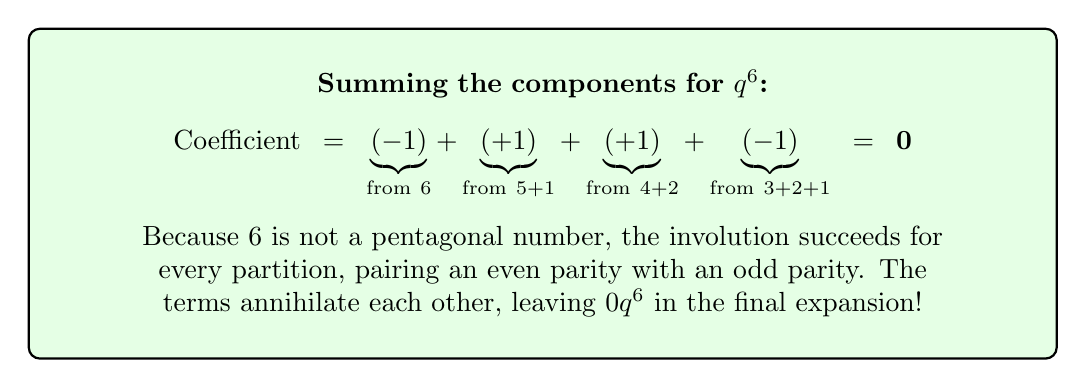
\begin{tikzpicture}
			\node[draw, thick, rounded corners, fill=green!10, inner sep=15pt, align=center, text width=12cm] {
				\textbf{Summing the components for $q^6$:} \\[0.3cm]
				$\text{Coefficient} = \underbrace{(-1)}_{\text{from } 6} + \underbrace{(+1)}_{\text{from } 5+1} + \underbrace{(+1)}_{\text{from } 4+2} + \underbrace{(-1)}_{\text{from } 3+2+1} = \mathbf{0}$ \\[0.3cm]
				Because $6$ is not a pentagonal number, the involution succeeds for every partition, pairing an even parity with an odd parity. The terms annihilate each other, leaving $0q^6$ in the final expansion!
			};
		\end{tikzpicture}
	\end{center}
	
\end{document}